\documentclass[20pt]{article}
\usepackage{graphicx}
\begin{document}

\title{%
  CSE 344 - System Programming \\
  \large Homework \#2}

\author{Harun ALBAYRAK - 171044014}

\maketitle

\Large
\section{How did I solve this problem?}
After I check this situation, I opened the file in read mode.
I get the file name from the first argument.
\\\\
After that, I created 8 processes for each row. These processes firstly go into "work" function. In the "work" function, I lock the file so that the other processes can't access. Then the process go into "calculate" function. In the "calculate" function, the given problem in the assignment is calculated. And the calculated values are written to end of related line. And after this,  I unlock the file so that the other processes can access.
\\\\
Each process do that work. Then, after it finishes the works the all processes send a SIGUSR1 signal to the parent processes. The SIGUSR1\_COUNT are increment to by 1 through these signals' handler. And the all child processes are suspended by SIGSUSPEND function.
\\\\
And while all these processes is happen, the parent processes is suspended by SIGSUSPEND function until SIGUSR1\_COUNT is 8. After SIGUSR1\_COUNT is 8, the average error of degree 5 is calculated by the "calculateAverageError" function. After that, the parent process send a SIGUSR2 signal to the all child processes. And the parent waits until its children are died.
 \\\\
The children that got a SIGUSR2 signal do the second stage. In this stage, the children calculate the 6 degree of Lagrange polynomial and prints out the coefficients of the polynomial. After doing its works, the children are died by the "\_exit" function.
\\\\
So, after the its children are died, the waiting of the parent process is finished. The average error of degree 6 is calculated by the "calculateAverageError" function. So the program is finished.  

\section{My Design Decisions}
I keep a SIGUSR1\_COUNT and SIGUSR2\_COUNT. Apart from that i keep all the children pids because i send SIGUSR2 signal.
\\\\
In the signal handler if the signal is SIGUSR1, i increment the SIGUSR1\_COUNT. And if the signal is SIGUSR2, i increment the SIGUSR2\_COUNT.

\section{Requirements I achieved and which I have failed}
I think I achieved almost all the requirements. However, I may not have been able to achieve some requirements.

\section{My Files}
171044014\_helper\_hw2.h $\Rightarrow$ The helper functions \\
171044014\_hw2.c $\Rightarrow$ The Main C File \\
171044014\_report.pdf $\Rightarrow$ The Report PDF \\
171044014\_report.tex $\Rightarrow$ The Report Latex file \\
Makefile $\Rightarrow$ The Makefile \\

\section{Some screenshots from the program}
\begin{figure}[h!]
  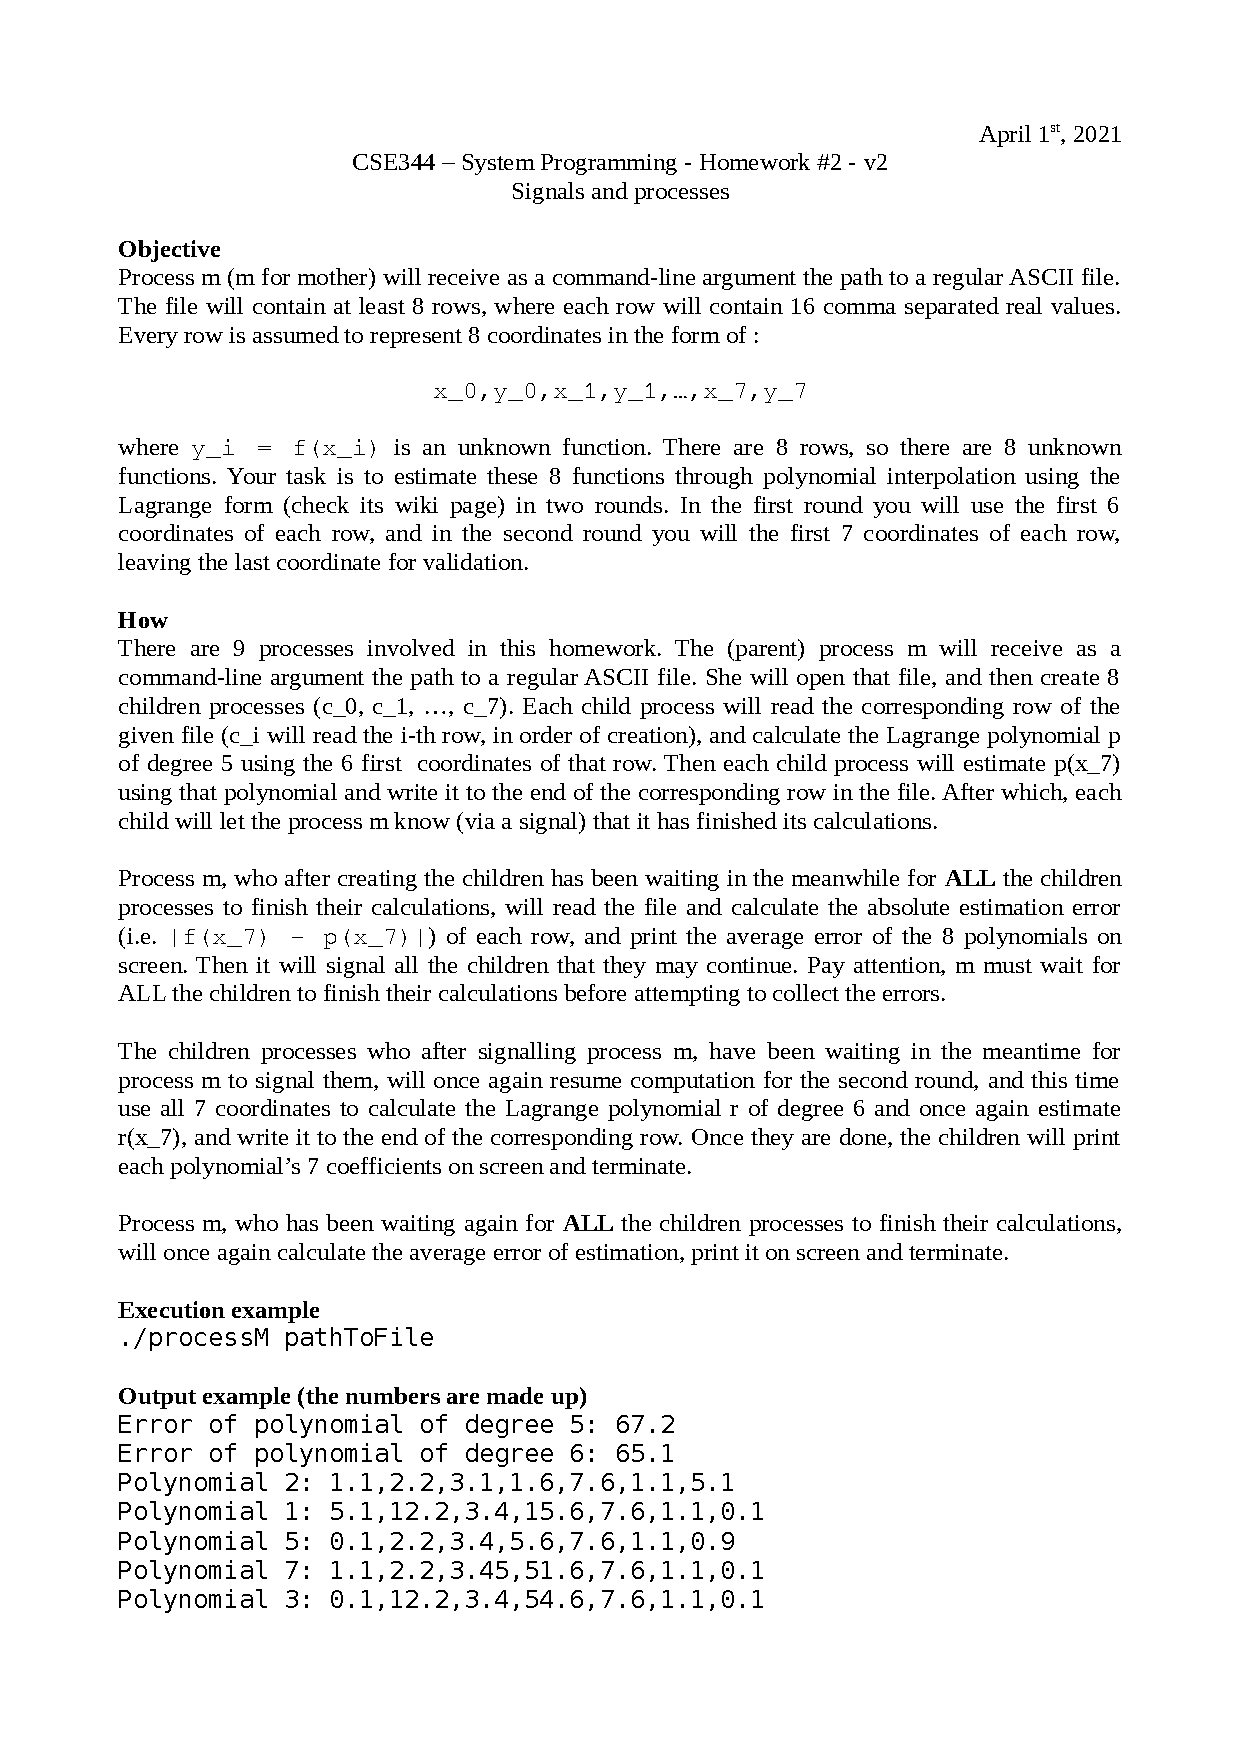
\includegraphics[width=\linewidth]{hw2.png}
  \caption{The output}
  \label{fig:code}
\end{figure}

\end{document}